% body.tex -- hand-maintained source of the manuscript (round-4 revision). Not generated.
\section{Introduction}

\IEEEPARstart{I}{n} early 2026, Hong Kong police reported more than 70 cases of a new traffic fraud: claimants filmed a driver crossing a solid line, reported the violation and, after the fine had been paid, demanded compensation for neck injuries, alleging that they had braked suddenly behind the driver~\cite{b1,b3}. Insurers described them as claims for accidents that never happened~\cite{b2}, and police later investigated over 100 suspicious cases, some without any impact~\cite{b60}. Similar schemes are recognized elsewhere: reports of suspected motor-insurance fraud in New York rose by 58\% from 2020 to 2023~\cite{b5}, and deliberate low-speed collisions (\emph{pengci}) are a long-standing form of extortion in China~\cite{b6}.

The accused vehicle is poorly equipped to answer such a claim. Event data recorders and data storage systems for automated driving (DSSAD) record around a trigger such as a crash~\cite{b7,b8}; without contact there is no trigger. Video recorders can run continuously~\cite{b9}, but loop recording overwrites footage long before a delayed claim arrives, a forward camera rarely sees the area behind the car, and long-term video retention raises privacy concerns. Above all, the driver must prove a negative: that a vehicle was \emph{not} in a specific place. Yet modern cars already carry rear-corner radars that observe exactly that place.

This paper asks what evidence a vehicle must keep, and how a verifier must read it, so that a later \emph{position} claim (``I was in your lane, between 2 and 30~m behind you, at 14:03'') can be refuted, supported or left open without refuting a genuine claim. We call this the \emph{proof-of-absence} problem and the resulting system PAL (Proof-of-Absence Ledger). ``Proof'' is used in the evidentiary sense: a refutation is a bounded-risk statement, not a certainty, and the term is unrelated to proofs of non-membership in authenticated data structures. It addresses fraud variants in which the claimed position is false---for example, a claimant who filmed from an adjacent lane or from farther back but claims to have been directly behind. Where the claimant really was behind the vehicle, the system supports the claim and the dispute moves to fault and injury, which radar position evidence cannot settle (Section~\ref{sec:verdict}).

\textbf{Research questions.}
\begin{enumerate}
\item[\textbf{RQ1.}] Can a vehicle refute delayed, no-contact position claims from its own radar data, without images, at practical storage and disclosure cost?
\item[\textbf{RQ2.}] Which system components keep wrong refutations (rejecting a genuine claim) and wrong supports (accepting a fabricated one) near zero?
\item[\textbf{RQ3.}] Does an explicit bound on the probability of missing the claimed vehicle (a \emph{formal tier}) make fewer wrong refutations than detection rules (a \emph{rule tier}) under sensing conditions that neither was designed for?
\item[\textbf{RQ4.}] Does the system resist a dishonest vehicle owner who manipulates sensors or the free-space record?
\end{enumerate}

\textbf{Contributions.}
\begin{enumerate}
\item A formulation of delayed, offline, adversarial position claims as a proof-of-absence problem, with a threat model that includes a dishonest owner (Section~\ref{sec:problem}).
\item An evidence system that derives a road-frame zone and a clock-bounded window from the claim, excludes sensors by attestation and liveness, records evidential free space per angular sector at higher resolution around the vehicle's own detected violation, and seals the record in a signed ledger from which only the zone's sectors are disclosed, with a completeness check that lets the verifier detect any withheld sample, sector or block---the non-omission property on which a negative claim rests (Section~\ref{sec:method}).
\item Two refutation tiers---detection rules, and a miss-probability bound whose soundness is stated in three propositions---in which sensor health is a precondition for refutation, combined into a graded verdict (Sections~\ref{sec:problem}--\ref{sec:theory}).
\item A simulation study with ablations, 13 degradation conditions, owner attacks, an integrity test of the ledger, a calibration of the bound against the ray-traced simulator, a pre-registered generalization test, in which the formal tier showed no measurable safety advantage over the rule tier, and exploratory stress tests of the assumptions, in which only the formal tier abstained on space hidden by an occluder (Sections~\ref{sec:setup}--\ref{sec:results}).
\end{enumerate}

\textbf{Scope.} The system judges only whether a vehicle was in the claimed zone during the claimed window. It does not judge fault, speed, injury or intent, and it identifies no road user. All results are simulated; Section~\ref{sec:realworld} sets out what real radar data must show.

\section{Related Work}\label{sec:related}

\textbf{Search protocol.} Literature and patents were searched in two rounds in 2026 with Google Scholar, arXiv, IEEE Xplore abstracts, Google Patents, the USPTO and Justia, combining the terms vehicle evidence, insurance fraud, staged or induced collision, \emph{pengci}, no-contact accident, free space, negative information, misbehavior detection, collective perception, sensor blockage, tamper-evident log and selective disclosure. Only~\cite{b24} was read claim by claim; other patents were assessed from abstracts, claims and descriptions. No professional patent database and no full-text Chinese, Japanese or Korean search was used, so the novelty statements below are provisional.

\textbf{Crash-triggered and continuous recording.} Event data recorders and DSSAD record around a trigger and, for DSSAD, document which agent controlled the vehicle~\cite{b7,b8}. Impact-triggered evidence capture~\cite{b10}, recorders of autonomous vehicles that keep buffers around events~\cite{b12}, recorders aimed at scams that show whether contact occurred~\cite{b14} and recorders triggered by the vehicle's own lane-departure warning~\cite{b17,b18} all assume an event and keep raw data around it. A claim submission that triggers a spatio-temporal query of nearby devices within a radius~\cite{b15}, and the comparison of vehicle data with an accident claim~\cite{b16}, are the closest claim-driven designs. Continuous surround recording as legal evidence is also patented~\cite{b9}.

\textbf{Free space, occlusion and negative information.} Evidential occupancy grids separate occupied, free and unknown space, so that occlusion is not mistaken for emptiness~\cite{b19}; grid handling, occlusion-aware occupancy and object-free-space detection are patented for vehicles and for mixed-reality devices~\cite{b20,b22,b23}. Search theory gives the probability that a target is present after an unsuccessful search, $P_{\mathrm{after}} = P_{\mathrm{before}}(1-\mathrm{POD})$, with POD the probability of detection~\cite{b30,b31}, and tracking exploits ``negative'' sensor evidence~\cite{b32}. None of these keeps free space as evidence for a later dispute.

\textbf{Plausibility of third-party position claims.} Vehicle-to-everything (V2X) misbehavior detection checks positions reported by other road users against the receiver's own perception. Intel's patents flag a reported object located in space that the receiver's sensors show as free~\cite{b24,b25}; Qualcomm's flag reported objects that the receiver's sensors fail to detect, weighted by sensor confidence~\cite{b26,b27}; Tischler and Vogt fuse observed-and-empty areas, kept apart from unobserved ones, for cooperative plausibility checks~\cite{b28}; and the ETSI collective perception message carries perceived objects together with sensor and perception-region information~\cite{b29}. These methods check a reported position, which is itself a claim, but they work live, on broadcast messages from cooperating road users, keep no evidence and do not bound the probability of a miss.

\textbf{Sensor health.} Radar blockage detection from the overlapping visibility of a neighboring radar---a sensor that misses targets its neighbor reports is declared blocked---is patented by Valeo Radar Systems~\cite{b33} and anticipates the liveness test used here.

\textbf{Accountable logs and selective disclosure.} Forensic and accountable logging frameworks make vehicle logs tamper-evident~\cite{b34,b35}; for autonomous IT operations, provable event non-occurrence has been shown for complete, anchored logs~\cite{b36}; zero-knowledge proofs let vehicles prove properties of cooperative-perception data~\cite{b37,b38}. A recorder specification for automated vehicles combines Merkle trees, Ed25519 and RFC~3161 anchoring~\cite{b39}, separate hash chains allow partial disclosure of evidence data~\cite{b40}, and salted-digest selective disclosure is standardized for credentials~\cite{b41}. Transparency logs prove inclusion and consistency of entries in Merkle trees~\cite{b62}; what a negative claim needs in addition is that nothing in a time window was left out of a disclosure. Table~\ref{tab:positioning} compares these lines of work.

\begin{table*}[!t]
\centering
\footnotesize
\caption{Positioning Against Related Work}
\label{tab:positioning}
\renewcommand{\arraystretch}{1.15}
\begin{tabular}{>{\raggedright\arraybackslash}p{4.4cm}>{\raggedright\arraybackslash}p{2.4cm}>{\raggedright\arraybackslash}p{2.6cm}>{\raggedright\arraybackslash}p{2.1cm}>{\raggedright\arraybackslash}p{2.1cm}>{\raggedright\arraybackslash}p{2.0cm}}
\toprule
\textbf{Capability} & \textbf{Event recorders \cite{b7,b8,b9,b10,b12,b14,b15,b16,b17,b18}} & \textbf{Free space, search theory \cite{b19,b20,b22,b23,b30,b31,b32}} & \textbf{V2X misbehavior \cite{b24,b25,b26,b27,b28,b29}} & \textbf{Accountable logs \cite{b34,b35,b36,b37,b38,b39,b40,b41}} & \textbf{This work} \\
\midrule
Works without contact or trigger & Partly \cite{b17,b18} & n/a & Yes (live) & Yes & Yes \\
Driven by a later third-party claim & Partly \cite{b15,b16} & No & No & No & Yes \\
Zone derived from the claim in road coordinates & No (radius \cite{b15}) & No & Live check of a reported position & No & Yes, offline \\
Observed-free vs.\ unobserved distinguished & No & Yes & Yes \cite{b28} & No & Yes (formal tier) \\
Bounded miss probability for refutation & No & Theory only \cite{b30} & No & No & Yes (formal tier) \\
Sensor health decides what may be refuted & No & Partly & Partly \cite{b26} & No & Yes (liveness as in \cite{b33}) \\
Tamper-evident, sector-level disclosure & No & No & No & Partly \cite{b39,b40,b41} & Yes (free-space record) \\
Completeness (non-omission) of a disclosure checked & No & No & No & Partly \cite{b36,b62} & Yes (free-space record) \\
\bottomrule
\multicolumn{6}{l}{\scriptsize n/a: not applicable.}
\end{tabular}
\end{table*}

\textbf{What is not novel.} Continuous recording as evidence~\cite{b9}; free, occupied and unknown representations and occlusion reasoning~\cite{b19,b20,b22,b23}; the search-theory update after an unsuccessful search~\cite{b30}; refuting a reported object because the receiver sees its location as free~\cite{b24,b25}; liveness by overlapping visibility~\cite{b33}; Merkle trees, Ed25519 signatures, hash chains, external anchors and salted selective disclosure~\cite{b39,b40,b41,b42,b43,b44}; and recording triggered by the vehicle's own lane departure~\cite{b17}. Nor is checking a reported position against observed free space as such~\cite{b24,b25,b28}. The contribution is the system that ties these parts to a delayed, offline and adversarial third-party claim---the claim-derived road-frame zone, sensor health as a precondition for refutation, the two refutation tiers and the graded verdict, and sector-level selective disclosure whose completeness the verifier checks---together with evidence, including a null result and the stress tests that break it, on which parts carry the safety.

\section{Problem Formulation}\label{sec:problem}

\begin{table}[!t]
\centering
\footnotesize
\caption{Notation}
\label{tab:notation}
\renewcommand{\arraystretch}{1.1}
\begin{tabular}{>{\raggedright\arraybackslash}p{2.4cm}>{\raggedright\arraybackslash}p{5.5cm}}
\toprule
\textbf{Symbol} & \textbf{Meaning} \\
\midrule
$c$ & claim (\ref{eq:1}): lane $\ell$, gap range $[g_{\min}, g_{\max}]$, class $k$, time $t_c$, tolerance $\tau$ \\
$Z$, $Z^-$, $W$ & claimed zone, inset zone for support, time window \\
$\Delta_{\mathrm{clk}}$ & attested clock bound (0.3~s) \\
$e_t(i)$ & record (\ref{eq:4}) of sector $i$ at sample $t$: free range, hit flag, bearing bin, healthy-sensor count \\
$S_Z(t)$, $r_i^{\max}$ & sectors meeting the zone; farthest zone range in sector $i$ \\
$\delta$, $\gamma$, $k_s$ & free-space margin (0.5~m), support gate (1~m), support count (3) \\
$\mathrm{occ}(t)$, $\mathrm{free}(t)$, $\mathrm{cover}(W)$ & sample predicates (\ref{eq:5})--(\ref{eq:6}); sampling of $W$ \\
$P_d$, $u$, $v$ & detection probability; persistent and per-sample fade \\
$\bar P_{\mathrm{miss}}(k, W)$, $\varepsilon$ & miss bound (\ref{eq:8}); its threshold ($10^{-3}$) \\
$r_t^{\max}$, $m_t$, $w^*$ & farthest zone range, minimum healthy-sensor count, worst weather at sample $t$ \\
\bottomrule
\end{tabular}
\end{table}

\textbf{Claim.} A claim filed against the ego vehicle is a tuple (\ref{eq:1})
\begin{equation}
c = (\ell,\; g_{\min},\; g_{\max},\; k,\; t_c,\; \tau)
\label{eq:1}
\end{equation}
where $\ell$ is the claimed lane as an absolute lane index of the road (the ego vehicle's own lane index is part of its pose log), $[g_{\min}, g_{\max}]$ the claimed longitudinal gap (front face of the claimant to the rear bumper of the ego vehicle, along the road), $k$ the claimed vehicle class, $t_c$ the claimed event time and $\tau$ the claimant's time tolerance. A claim asserts that the claimant was in the zone throughout the resulting window; a claimant who was there only briefly makes a weaker claim, which Section~\ref{sec:stress} examines. Claims arrive days or weeks later, so no live data, footage or witness can be assumed. Table~\ref{tab:notation} summarizes the notation.

\textbf{Zone and window.} The claim induces a road-frame zone (\ref{eq:2}) and a time window (\ref{eq:3})
\begin{align}
Z(c) &= \{(s,l) : s - s_{\mathrm{ego}} \in [-g_{\max}, -g_{\min}], \nonumber\\
&\qquad\quad |l - l_\ell| \le w_L/2\}, \label{eq:2}\\
W(c) &= [\,t_c - \tau - \Delta_{\mathrm{clk}},\; t_c + \tau + \Delta_{\mathrm{clk}}\,], \label{eq:3}
\end{align}
with $(s,l)$ the road-aligned arc-length and lateral coordinates, $s_{\mathrm{ego}}$ the arc length of the ego vehicle's rear bumper at the sample time, $l_\ell$ the lane center, $w_L$ the lane width and $\Delta_{\mathrm{clk}} = 0.3$~s the attested clock bound. The zone follows road curvature, taken as constant over the zone from the logged curvature, and is re-expressed in the ego frame of every logged sample through the logged pose; on clothoid road segments this extrapolation adds a lateral error that grows with $g_{\max}^3$. Returns used for \emph{support} must lie in an inset zone $Z^-$ (0.3~m laterally, 0.5~m longitudinally), so that returns from the adjacent lane or the zone edge cannot support a claim.

\textbf{Evidence record.} At each sample time $t$ and for each angular sector $i$ of width $\Delta\theta$, the vehicle stores
\begin{equation}
e_t(i) = (d_i,\; h_i,\; b_i,\; n_i),
\label{eq:4}
\end{equation}
where $d_i$ is the evidential free range---a deterministic range, not a Dempster--Shafer mass (the minimum, over healthy sensors and rays in the sector, of the range to the first return or to the field-of-view limit, quantized down to 0.5~m), $h_i \in \{0,1\}$ states whether that range ended in a return, $b_i$ is a 3-bit bearing bin of that return and $n_i$ the number of healthy sensors covering the sector. Space beyond $d_i$, and any sector with $n_i = 0$, is unknown, never free. Sectors are $2.5^\circ$ wide at 2~Hz by default and $1^\circ$ wide at 10~Hz for $\pm 10$~s around a self-detected solid-line crossing. The record holds no images, identities or object lists. A detection log (per-sensor detections at 10~Hz) is kept alongside it for the rule tier.

\textbf{Sample predicates.} For a sample $t \in W$, let $S_Z(t)$ be the sectors meeting the zone, $r_i^{\max}$ the farthest zone point in sector $i$ and $\delta = 0.5$~m. Then
\begin{align}
\mathrm{occ}(t) &\iff \exists\, i \in S_Z(t):\; h_i = 1 \wedge p_i \in Z^-(t), \label{eq:5}\\
\mathrm{free}(t) &\iff \forall\, i \in S_Z(t):\; n_i > 0 \;\wedge \nonumber\\
&\qquad \big[(h_i = 0 \wedge d_i + \delta \ge r_i^{\max}) \nonumber\\
&\qquad\; \vee\, (h_i = 1 \wedge d_i \ge r_i^{\max} + \delta)\big], \label{eq:6}
\end{align}
so a return counts as free space only when it lies at least $\delta$ beyond the zone, where $p_i$ is the point reconstructed from $d_i$ and $b_i$. In the no-return clause, $\delta$ absorbs the downward quantization of $d_i$ and of the zone grid; it departs from A2 (Section~\ref{sec:theory}), and Section~\ref{sec:calib} shows that removing it changes no verdict. $S_Z(t)$ and $r_i^{\max}$ are computed from zone points on a 0.5~m grid. The samples must also cover $W$, written $\mathrm{cover}(W)$: consecutive samples at most 1.5 sampling periods apart, and the first and last within 1.5 periods plus $\Delta_{\mathrm{clk}}$ of the window ends. The extra $\Delta_{\mathrm{clk}}$ means that the clock-uncertain margins of $W$ need not be sampled; it was introduced before the pre-registration freeze (Section~\ref{sec:setup}).

\textbf{Support.} Each tier tests support on its own evidence. Returns in $Z^-$ are expressed as (gap, lateral offset) in the zone's road frame at their own sample, and support requires a return matched within a gate $\gamma = 1$~m by returns from at least $k_s - 1 = 2$ other samples satisfying (\ref{eq:5}): in the free-space record for the formal tier and in the detection log for the rule tier. The test assumes that the claimant keeps roughly the ego vehicle's speed; a claimant whose gap changes by more than $\gamma$ between matched samples is not supported, and the verdict then falls back to the refutation tests. SUPPORTED means that \emph{a} vehicle was observed in the claimed zone; radar does not verify the claimed class.

\textbf{Rule tier.} The rule tier refutes when every zone point lies in the field of view of a healthy sensor at every sample of $W$, no detection at all---even a single, non-persistent one---falls inside $Z$, and the claimed class is not a weak reflector (motorcycle claims are never refuted). It does not reason about occlusion.

\textbf{Formal tier.} The formal tier refutes when (\ref{eq:7}) holds: the samples cover $W$, every sample is free, and the probability that a genuine claimant of class $k$ would have been missed is bounded by $\varepsilon$:
\begin{multline}
V_{\mathrm{formal}}(c) = \text{REFUTED} \iff \\
\mathrm{cover}(W) \wedge \textstyle\bigwedge_{t \in W} \mathrm{free}(t) \wedge \bar P_{\mathrm{miss}}(k, W) \le \varepsilon,
\label{eq:7}
\end{multline}
where $\mathrm{cover}(W)$ is the sampling condition above, $\varepsilon = 10^{-3}$ a policy parameter (at most one wrong refutation per thousand genuine claims under the model), and $\bar P_{\mathrm{miss}}$ the bound of Section~\ref{sec:theory}, evaluated at the farthest zone range, the minimum sensor count over the zone and the most severe modeled weather, since the record stores no weather.

\textbf{Graded verdict.} A SUPPORTED from either tier overrides refutation. Otherwise the verdict is REFUTED (standard) when both tiers refute, REFUTED (weak) when only one does (the report names which) and INCONCLUSIVE when neither does; \emph{weak-or-better} denotes either kind of refutation. A weak refutation is reported as ``no vehicle detected'', not as proof of absence, and a refutation by the rule tier alone is marked as resting on unsealed evidence until the detection log is integrity-protected (Section~\ref{sec:method}). A disclosure that fails the integrity or completeness checks of Section~\ref{sec:method} is INVALID.

\textbf{Metrics.} Ground truth is \emph{genuine} when a vehicle at least as detectable as the claimed class has its front face in the gap range, within 1~m of the claimed lane center, at the claimed event time, and \emph{empty} when no vehicle body overlaps the zone at any time in $W$. Claims that are neither (a smaller vehicle in the zone, or a partial or off-time overlap) are reported separately. The metrics compare verdicts with simulator ground truth: the wrong-refutation rate $P(\text{REFUTED}\mid\text{genuine})$, the safety-critical error; the wrong-support rate $P(\text{SUPPORTED}\mid\text{empty})$; the coverage $P(\text{REFUTED}\mid\text{empty})$, i.e., the share of fabricated claims that can be refuted; and the support and inconclusive rates on genuine claims.

\textbf{Threat model.} (i) A \emph{claimant} who fabricates position, lane and time, may place a real vehicle near but not in the zone, chooses the claimed class and gap freely and cannot alter the record. (ii) A \emph{dishonest owner} who wants a genuine claim refuted: the owner may cover or rotate a sensor, shift the clock, edit or withhold parts of the free-space record, or obtain the signing key; key compromise before the next anchor is published is not covered, and the detection log is not yet protected (Section~\ref{sec:method}). Logger firmware is assumed to run under measured boot, and the hardware security module signs only blocks that the logger seals; a compromised logger is equivalent to a compromised key. A shifted clock is countered by aligning the claimed time with the vehicle's own recorded solid-line crossing, which the claimant's video also shows; this alignment was not simulated, because simulated claims always refer to the crossing. (iii) A \emph{privacy attacker} who obtains disclosed records (Section~\ref{sec:privacy}). Physical spoofing of radar returns is out of scope.

\section{Theory of the Formal Tier}\label{sec:theory}

This section states what a formal-tier refutation guarantees and under which assumptions. Section~\ref{sec:calib} tests the guarantee against the ray-traced simulator.

\needspace{6\baselineskip}
\textbf{Assumptions.}
\begin{itemize}
\item \emph{A1 (conservative storage).} $d_i$ is the minimum over the sensor rays falling in sector $i$ of the range to the first return or to the field-of-view limit, quantized down; $n_i$ counts only sensors that passed attestation and liveness and whose rays meet every vehicle lying in the zone part of the sector. The implementation counts a sensor with at least one ray in the sector, which can overstate $n_i$ in sectors cut by the edge of a field of view.
\item \emph{A2 (range margin).} Every counted sensor's range limit is at least $r_i^{\max} + \delta$ in each zone sector.
\item \emph{A3 (pose, bearing and clock).} Pose and sensor-bearing errors are small against the insets and $\delta$, and rays are cast from a common origin; clock error is within $\Delta_{\mathrm{clk}}$. The attested calibration residual admits up to $2^\circ$ of bearing error, 1.7~m laterally at 48~m, which exceeds the 0.3~m inset; the implementation does not widen the zone by it, and the simulator ignores mounting offsets.
\item \emph{A4 (first object).} Any object on a ray between the ego vehicle and a genuine claimant is at least as detectable as the claimed class, including its fading.
\item \emph{A5 (detection model $M$).} Detection of an object of class $k$ at range $r$ is Bernoulli with probability $P_d = \Lambda(\mathrm{SNR}/\beta)$, where $\Lambda$ is the logistic function and the signal-to-noise ratio is $\mathrm{SNR} = \mathrm{snr}_0 + \mathrm{RCS}_k - 40\log_{10}(r/r_0) - L_w + u + v$, with $\mathrm{RCS}_k$ the radar cross-section of class $k$, $r_0 = 80$~m, weather loss $L_w$, a persistent fade $u \sim \mathcal{N}(0,\sigma_u^2)$ shared by all samples of the event and an independent per-sample, per-sensor fade $v \sim \mathcal{N}(0,\sigma_v^2)$.
\item \emph{A6 (presence).} A genuine claimant is in the zone during every sample of $W$, as the claim asserts.
\end{itemize}

\begin{proposition}[Visibility soundness]\label{prop:1}
Under A1--A3, if sample $t$ is free and a vehicle $V$ lies in $Z$ at time $t$, then on every healthy ray that meets $V$ at a point of $Z$ the first object along the ray was not detected by that sensor at $t$.
\end{proposition}
\begin{IEEEproof}
Take a healthy ray $\rho$ in sector $i$ meeting $V$ at a point of $Z$, at range $r \le r_i^{\max}$, and suppose that $\rho$ returned from its first object at $r' \le r$. Since $d_i$ is the minimum over the sector's rays, $d_i \le r' \le r_i^{\max}$. If the sector minimum is a return, $h_i = 1$ and (\ref{eq:6}) requires $d_i \ge r_i^{\max} + \delta$, a contradiction. Otherwise the minimum is a ray ending at its range limit, which is then at most $r' \le r_i^{\max}$, contradicting A2. Hence no return occurred on $\rho$ before $V$.
\end{IEEEproof}

A2 is not enforced by the implementation, which accepts a no-return sector when $d_i + \delta \ge r_i^{\max}$; the gap matters only when the zone ends within $\delta$ beyond a sensor's range limit. Section~\ref{sec:calib} reports a sensitivity check with a tightened clause.

\begin{proposition}[Miss bound]\label{prop:2}
Under A1--A6, the probability that every sample of $W$ is free for a genuine claimant of class $k$ is at most
\begin{multline}
\bar P_{\mathrm{miss}}(k, W) = \int \phi(u; 0, \sigma_u^2) \\
\times \prod_{t \in W} \Big[ \mathbb{E}_v\big(1 - P_d(k, r_t^{\max}, w^*, u, v)\big) \Big]^{m_t} du ,
\label{eq:8}
\end{multline}
where $r_t^{\max}$ is the farthest zone range, $m_t$ the minimum healthy-sensor count over the zone sectors at sample $t$ and $w^*$ the most severe modeled weather. Hence the formal tier wrongly refutes with probability at most $\varepsilon$ under $M$.
\end{proposition}
\begin{IEEEproof}
By Proposition~\ref{prop:1}, a free sample requires every covering healthy sensor to miss the first object on its rays. By A4 that object is no easier to miss than class $k$ at $r_t^{\max}$, since $P_d$ decreases with range and weather loss. Conditional on $u$, misses are independent across sensors and samples (A5), so the joint probability is at most the product over samples of the per-sample miss probability to the power $m_t$, averaged over $v$. Integrating over $u$ gives (\ref{eq:8}).
\end{IEEEproof}

The integrals use 24-point Gauss--Hermite quadrature. The persistent fade $u$ is why a long window does not drive the bound to zero: a claimant that reflects weakly throughout the event is not rescued by more samples.

\begin{proposition}[Monotonicity of the bound]\label{prop:3}
For a fixed set of free samples, $\bar P_{\mathrm{miss}}$ is non-increasing in the number of samples and in each $m_t$, and non-decreasing in each $r_t^{\max}$ and in $L_w$.
\end{proposition}
\begin{IEEEproof}
Each factor lies in $[0,1]$, and $P_d$ increases with SNR. Integration over $u$ preserves the order.
\end{IEEEproof}

Proposition~\ref{prop:3} concerns the bound only. It does not imply that more samples or narrower sectors make refutation more likely, because each extra sample must itself be free. Enrichment therefore cuts both ways (Section~\ref{sec:ablation}).

\textbf{Limits.} The guarantee is conditional on $M$ and on A1, which the implementation meets only approximately; where it counts a sensor whose rays miss part of the zone, $m_t$ overstates the independent looks and (\ref{eq:8}) is no longer an upper bound. A4 fails when a less detectable object (for example a motorcycle) shields a larger claimed vehicle, and the positive association of the first object's fade with the claimant's is assumed, not proven. A6 fails when the claimant enters or leaves the zone within the window. Real per-sample fade correlation at 10~Hz is unknown. Against the ray-traced simulator the bound held under the matched model and was optimistic for cars once returns were about 9~dB weaker than modeled (Section~\ref{sec:calib}); Section~\ref{sec:stress} tests fades that are correlated over time and claimants that leave the zone.

\section{Method}\label{sec:method}

\textbf{Architecture.} The system runs as a passive logger in the vehicle and as an offline verifier at the insurer or court (Fig.~\ref{fig:arch}). It reads the ego pose, sensor self-diagnostics, lane-line detections and, per radar, a clearance for every azimuth---the range to the first return or to the field-of-view limit. Sparse detection lists after constant-false-alarm-rate processing do not provide that clearance directly; a radar free-space output or an inverse sensor model must supply it. It never controls the vehicle.

\begin{figure*}[!t]
\centering
\begin{tikzpicture}[font=\footnotesize,
  box/.style={draw=#1, rounded corners=2pt, align=center, minimum height=8mm, inner sep=3pt, fill=#1!12, line width=0.6pt},
  box/.default=palblue,
  src/.style={align=right, anchor=east, inner sep=1pt, text=palink2},
  arr/.style={-{Stealth[length=2mm]}, line width=0.7pt, draw=palink2}]
\fill[palblue!5] (-1.7,2.75) rectangle (9.55,-3.05);
\fill[palmuted!9] (11.35,2.75) rectangle (15.8,-3.05);
% inputs
\node[src] (pose) at (0.9,1.7) {ego pose, clock};
\node[src] (lane) at (0.9,0.85) {lane-line events};
\node[src] (radar) at (0.9,-1.3) {azimuth clearance\\+ detections\\(per radar)};
% processing
\node[box=palmuted, text width=2.9cm] (enr) at (3.2,0.85) {\textbf{2} enrichment trigger:\\own solid-line crossing};
\node[box=palmuted, text width=2.6cm] (att) at (3.2,-1.3) {\textbf{1} sensor attestation\\+ liveness};
% ledger frame around the free-space record
\draw[palaqua, fill=palaqua!10, rounded corners=3pt, line width=0.8pt] (5.2,1.3) rectangle (9.4,-0.85);
\node[box=palaqua, text width=2.8cm] (rec) at (7.3,0.62) {\textbf{3} free-space record\\$e_t(i)=(d_i,h_i,b_i,n_i)$ + ego leaf};
\node[align=center, font=\scriptsize, text=palink] at (7.3,-0.42) {\textbf{4} ledger: salted leaves, Merkle tree,\\hash chain, Ed25519 (HSM), anchor};
\node[box=palaqua, dashed, text width=2.8cm] (dlog) at (7.3,-2.1) {\textbf{3$'$} detection log\\(per-sensor detections)};
% offline column
\node[box=palmuted, text width=3.3cm] (v1) at (13.55,1.7) {\textbf{6} claim $\rightarrow$ zone $Z$, window $W$};
\node[box=palmuted, below=2.6mm of v1, text width=3.3cm] (v2) {\textbf{7} integrity + completeness};
\node[box=palmuted, below=2.6mm of v2, text width=3.3cm] (v3) {\textbf{8} support (persistent returns in $Z^-$)};
\node[box=palblue, text width=1.42cm, anchor=north west] (v4a) at ([yshift=-2.6mm]v3.south west) {\textbf{9} rule\\tier};
\node[box=palorange, text width=1.42cm, anchor=north east] (v4b) at ([yshift=-2.6mm]v3.south east) {\textbf{9} formal\\tier};
\path (v4a.south) -- (v4b.south) coordinate[midway] (m45);
\node[box=palmuted, text width=3.3cm, anchor=north] (v5) at ([yshift=-2.6mm]m45) {\textbf{10} graded verdict};
% arrows (in the vehicle)
\draw[arr] (pose.east) -- (7.3,1.7) -- (rec.north);
\draw[arr] (lane) -- (enr);
\draw[arr] (enr.east) -- (rec.west |- enr.east);
\draw[arr] (radar) -- (att);
\draw[arr] (att.east) -- (4.95,-1.3) |- ([yshift=-2mm]rec.west);
\draw[arr] (4.95,-1.3) |- (dlog.west);
% disclosure and detection log to the verifier
\draw[arr, draw=palaqua!80!black] (9.4,0.62) -- (10.95,0.62) |- (v2.west);
\node[font=\scriptsize, text=palink, align=center, anchor=north] at (10.45,0.5) {\textbf{5} disclose\\zone sectors\\in $W$};
\draw[arr, dashed] (dlog.east) -- (11.1,-2.1) |- (v4a.west);
\draw[arr, dashed] (11.1,-2.1) |- (v3.west);
\node[font=\scriptsize, text=palink2, align=left, anchor=north west] at (8.95,-2.2) {not yet sealed};
\draw[arr] (v1) -- (v2); \draw[arr] (v2) -- (v3);
\draw[arr] (v3.south -| v4a.north) -- (v4a.north); \draw[arr] (v3.south -| v4b.north) -- (v4b.north);
\draw[arr] (v4a.south) -- (v4a.south |- v5.north); \draw[arr] (v4b.south) -- (v4b.south |- v5.north);
\node[font=\footnotesize\bfseries, text=palblue!70!black, anchor=north west] at (-1.6,2.7) {IN THE VEHICLE (continuous, no images)};
\node[font=\footnotesize\bfseries, text=palink2, anchor=north] at (13.55,2.7) {OFFLINE VERIFIER, AFTER A CLAIM};
\end{tikzpicture}
\caption{System architecture. In the vehicle (blue background), attested sensors feed a sector-level free-space record and a detection log (aqua); the record, with an ego leaf per sample, is densified around the vehicle's own solid-line crossing and sealed in a signed ledger (aqua frame). After a claim (gray background), only the zone's sectors in the window are disclosed; the verifier derives the zone and window from the claim, checks integrity and completeness (no withheld or repeated evidence), tests support, and evaluates the rule tier (blue) and the formal tier (orange), which form the graded verdict. The detection log, read by the support test and the rule tier, is not yet integrity-protected (dashed).}
\label{fig:arch}
\end{figure*}


\textbf{1) Attestation and liveness.} A sensor is excluded when its blockage flag is set or its calibration residual exceeds $2^\circ$. Because a blockage flag can be missed, a sensor that reports no return in the window while another sensor reports returns inside its field of view is also excluded (overlapping-visibility liveness, as in~\cite{b33}). Excluded sensors contribute $n_i = 0$, so their space is unknown, never free, and their field of view does not count as covered for the rule tier. In the simulation the liveness test uses the whole $\pm 1.3$~s window; a deployed logger needs a trailing window.

\textbf{2) Enrichment.} When the vehicle's own lane-keeping function detects a solid-line crossing---the trigger of the reported scam---the free-space record switches for $\pm 10$~s from $2.5^\circ$ at 2~Hz to $1^\circ$ at 10~Hz.

\textbf{3) Records.} The free-space record holds (\ref{eq:4}) per sector in two bytes---one for the free range (0.5~m steps, capped at 127.5~m) and one for the hit flag, bearing bin and healthy-sensor count---plus a 40-byte ego leaf per sample (time, arc length, lateral offset, relative heading and curvature). The detection log holds per-sensor detections for the rule tier.

\textbf{4) Ledger.} Every sample becomes one ego leaf and one leaf per sector. Leaf $j$ of a block is hashed with its index and a 128-bit salt derived as $\mathrm{HMAC\text{-}SHA256}(\text{seed}, j)$; only the 32-byte block seed is stored, inside the hardware security module (HSM) with the signing key, so that disclosing a leaf reveals its own salt but nothing about undisclosed 2-byte leaves. The leaves of a 60~s block form a Merkle tree~\cite{b42}; the block header holds the root, the block's time range, the hash of the layout (time and sector count of each sample) and the hash of the previous header, and is signed with Ed25519~\cite{b43}. Once per hour of driving, only the latest 32-byte header hash leaves the vehicle, to be time-stamped (RFC~3161~\cite{b44}) or stored by the manufacturer. The ledger was implemented and tested for the free-space record only; the detection log used by the rule tier is not yet integrity-protected; its storage is only estimated (Section~\ref{sec:discussion}) and its disclosure cost was not measured.

\textbf{5) Disclosure.} For a claim, the owner discloses the ego leaves and zone sectors of every sample in $W$ with their salts, one Merkle multiproof per block, the layout of each disclosed block and the headers from the last block that ends before $W$ to the anchor.

\textbf{6)--10) Verification.} The verifier checks the signatures, the hash chain to the anchor and the Merkle roots; recomputes, from the claim and the disclosed ego leaves, which sectors the zone touches; and rejects the disclosure as INVALID if the header chain starts inside $W$, if any sample of $W$, any required sector or any block whose signed time range overlaps $W$ is missing, or if a block, leaf or sample is repeated. A gap in the logger's own sampling is not a withholding: the disclosure is then valid, $\mathrm{cover}(W)$ fails and the formal tier cannot refute. It then tests support and evaluates both refutation tiers and the graded verdict (Algorithm~\ref{alg:verify}, Fig.~\ref{fig:block}).

\begin{algorithm}[!t]
\caption{Verification of a Claim}
\label{alg:verify}
\footnotesize
\begin{algorithmic}[1]
\Require claim $c$; disclosure $D$; anchor $A$; public key $K$; detection log $L$ (not yet sealed); $\varepsilon=10^{-3}$, $k_s=3$, $\gamma=1$~m, $\delta=0.5$~m
\State $Z, W \gets$ zone and window of $c$, (\ref{eq:2})--(\ref{eq:3})
\If{a signature (with $K$), the hash chain to $A$ or a Merkle root fails}
  \State \Return INVALID
\EndIf
\If{the chain starts inside $W$; a block overlapping $W$, a logged sample of $W$ or a zone sector is withheld; or a block, leaf or sample is repeated}
  \State \Return INVALID \Comment{withheld evidence}
\EndIf
\For{each sample $t \in W$}
  \State $Z_t \gets$ zone of $c$ in the disclosed ego pose; $S_t \gets$ sectors meeting $Z_t$
  \State $H_t \gets$ hits of $S_t$ in $Z_t^-$;\; $\mathrm{free}_t \gets$ all of $S_t$ satisfy (\ref{eq:6})
\EndFor
\If{$\bigcup_t H_t$ persists ($k_s,\gamma$) or detections of $L$ in $\bigcup_t Z_t^-$ persist} 
  \State \Return SUPPORTED
\EndIf
\State $R_{\mathrm{rule}} \gets$ $Z$ covered by healthy sensors at all $t$
\Statex \hspace{\algorithmicindent}\quad $\wedge$ no detection of $L$ in $Z$ $\wedge$ class $\neq$ motorcycle
\State $R_{\mathrm{formal}} \gets$ samples cover $W$ $\wedge$ $\bigwedge_t \mathrm{free}_t$
\Statex \hspace{\algorithmicindent}\quad $\wedge\; \bar P_{\mathrm{miss}}(k, W) \le \varepsilon$ \Comment{(\ref{eq:8})}
\If{$R_{\mathrm{rule}} \wedge R_{\mathrm{formal}}$} \State \Return REFUTED (standard)
\ElsIf{$R_{\mathrm{rule}} \vee R_{\mathrm{formal}}$} \State \Return REFUTED (weak), naming the tier
\EndIf
\State \Return INCONCLUSIVE
\end{algorithmic}
\end{algorithm}


\begin{figure}[!t]
\centering
\resizebox{\columnwidth}{!}{%
\begin{tikzpicture}[font=\footnotesize,
  stp/.style={draw=palmuted, fill=palmuted!12, rounded corners=2pt, align=center, minimum height=7mm, text width=3.3cm, line width=0.6pt},
  tier/.style={draw=#1, fill=#1!12, rounded corners=2pt, align=center, minimum height=11mm, text width=2.9cm, line width=0.6pt},
  out/.style={draw=#1, fill=#1!18, rounded corners=2pt, align=center, minimum height=6.5mm, text width=2.3cm, line width=0.8pt, font=\footnotesize\bfseries},
  q/.style={font=\footnotesize\itshape, text=palink2},
  arr/.style={-{Stealth[length=1.6mm]}, line width=0.6pt, draw=palink2}]
\node[stp] (s1) at (0,0) {integrity: signatures, hash chain to anchor, Merkle roots};
\node[stp] (s2) at (0,-1.2) {completeness: every sample of $W$ and every sector of the claim's zone};
\node[stp] (s3) at (0,-2.45) {support (either tier): $\ge k_s$\\samples with returns in $Z^-$};
\node[out=palcritical] (inv) at (3.55,-0.6) {INVALID};
\node[out=palgood] (sup) at (3.55,-2.45) {SUPPORTED};
\node[tier=palblue] (rt) at (-1.7,-4.15) {\textbf{rule tier}\\$Z$ covered, no detection in $Z$, not a motorcycle};
\node[tier=palorange] (ft) at (1.7,-4.15) {\textbf{formal tier}\\$W$ covered, all samples free (\ref{eq:6}), $\bar P_{\mathrm{miss}}\le\varepsilon$};
\node[draw=palink2, fill=white, rounded corners=2pt, align=center, minimum height=6mm, text width=2.6cm, line width=0.6pt] (cmb) at (0,-5.6) {how many tiers refute?};
\node[out=palviolet, text width=2.0cm] (std) at (-2.6,-7.15) {REFUTED (standard)};
\node[out=palyellow, text width=2.1cm] (wk) at (0,-7.15) {REFUTED (weak),\\tier named};
\node[out=palmuted, text width=2.2cm] (inc) at (2.6,-7.15) {INCONCLUSIVE};
\draw[arr] (s1) -- (s2); \draw[arr] (s2) -- (s3);
\draw[arr] (s1.east) -| node[q, pos=0.25, above]{fail} (inv.north);
\draw[arr] (s2.east) -| node[q, pos=0.25, below]{missing, repeated} (inv.south);
\draw[arr] (s3.east) -- node[q, above, pos=0.55]{yes} (sup.west);
\draw[arr] (s3.south) -- node[q, right, pos=0.45]{no} (0,-3.3) -| (rt.north);
\draw[arr] (0,-3.3) -| (ft.north);
\draw[arr] (rt.south) |- (cmb.west);
\draw[arr] (ft.south) |- (cmb.east);
\draw[arr] (cmb.south) -- ++(0,-1.5mm) -| node[q, pos=0.75, left]{both} (std.north);
\draw[arr] (cmb.south) -- node[q, left, pos=0.62]{one} (wk.north);
\draw[arr] (cmb.south) -- ++(0,-1.5mm) -| node[q, pos=0.75, right]{none} (inc.north);
\end{tikzpicture}}
\caption{Verdict logic of the verifier. Integrity or completeness failures make the disclosure invalid; persistent returns in the inset zone support the claim; otherwise the rule and formal tiers are evaluated independently: both refuting gives a standard refutation, one a weak refutation, none an inconclusive verdict. Gray marks steps shared by both tiers, blue the rule tier and orange the formal tier; outcomes are red (invalid), green (supported), violet (standard refutation), yellow (weak refutation) and gray (inconclusive), always with their label.}
\label{fig:block}
\end{figure}


\textbf{Cost.} Logging costs $O(N_{\mathrm{sec}} + R)$ per sample for $N_{\mathrm{sec}}$ sectors and $R$ returns. Verification costs $O(|W|\,|S_Z|)$ for the verdict, $O(|D| \log n)$ hashes for the multiproofs of a disclosure $D$ over blocks of $n$ leaves and $O(|W|\,Q^2)$ for the bound with $Q = 24$ quadrature nodes. Both tiers together took a median of 0.067~s per claim (10th--90th percentile 0.050--0.095~s, 100 claims) in unoptimized Python. Sizes are reported in Section~\ref{sec:attacks}.

\section{Experimental Setup}\label{sec:setup}

All results are \emph{simulated}; no real sensor data were used.

\subsection{Simulator}
A purpose-built 2-D simulator reproduces the reported fraud pattern~\cite{b1,b2,b3}. On a three-lane road (lane width 3.5~m; straight, or curved with radius 300~m or 600~m) the ego vehicle changes lane across a solid line at $t = 0$, and a claim is filed for the lane it moves into, with a gap from 2~m to a 2~s headway at the claimed vehicle's speed and a tolerance of $\pm 1$~s; the claimed gaps therefore ended 24--48~m behind the vehicle (median 36~m), and short claims were not simulated separately. The claimant is placed in the zone in about half of the scenes; otherwise it stays nearby (in an adjacent lane at 3--30~m, or in the claimed lane at least 8~m beyond the gap). This distribution of fabricated claims is a modeling choice, and coverage figures are conditional on it. Traffic vehicles can also make a claim genuine, so 57.7\% of the main-benchmark scenes are genuine (Fig.~\ref{fig:pie}). A van directly behind the ego vehicle appears in 25\% of scenes; its body overlaps the near part of the zone. Vehicles are oriented boxes, and three radars are ray-traced exactly at $0.5^\circ$ and 10~Hz over $\pm 1.3$~s, with detection per A5 and the faults of Table~\ref{tab:sim}. The simulator alone holds ground truth; the methods see sensor output, the noisy ego log, self-diagnostics and the claim.

\begin{table*}[!t]
\centering
\footnotesize
\caption{Simulator Parameters (Nominal); All Values Are Assumptions of This Study}
\label{tab:sim}
\renewcommand{\arraystretch}{1.15}
\begin{tabular}{>{\raggedright\arraybackslash}p{6cm}>{\raggedright\arraybackslash}p{10.6cm}}
\toprule
\textbf{Parameter} & \textbf{Value} \\
\midrule
Radars (boresight, half field of view, range) & rear-left $135^\circ$, $\pm 75^\circ$, 80~m; rear-right $-135^\circ$, $\pm 75^\circ$, 80~m; front $0^\circ$, $\pm 50^\circ$, 160~m \\
SNR of a 0~dBsm target at $r_0 = 80$~m; logistic slope $\beta$ & $-7$~dB; 1.5~dB \\
Range loss & $40 \log_{10}(r/r_0)$ \\
Radar cross-section (RCS): car / van / truck / motorcycle & 10 / 15 / 20 / 0~dBsm$^{a}$ \\
Persistent fade $\sigma_u$; per-sample fade $\sigma_v$ & 4~dB; 3~dB \\
Weather: clear / rain / fog (loss; share) & 0 / 2.5 / 1~dB; 0.6 / 0.3 / 0.1 \\
Ego speed & 50--80~km/h \\
Claimed class & car 0.85, motorcycle 0.15 \\
Traffic & 0--6 vehicles; car 0.70, van 0.10, truck 0.05, motorcycle 0.15 \\
Ghost returns & 0.03 per radar per sample, 5--40~m, $\pm 0.75^\circ$ wide \\
Blockage (rear radars only) & probability 0.05; flag recall 0.95 \\
Misalignment (rear radars only) & probability 0.05; $4^\circ$--$10^\circ$; calibration noise $0.5^\circ$ \\
Clock offset; pose noise & $\sigma = 0.1$~s (0.3\% of scenes exceed $\Delta_{\mathrm{clk}}$); 0.05~m along, 0.10~m lateral, $0.3^\circ$ heading, $10^{-4}~\mathrm{m}^{-1}$ curvature \\
Lane-crossing detection recall & 0.95 (enriched record in 94.8\% of main-benchmark scenes) \\
Ego lane change & cosine lateral profile over $t \in [-2, 2]$~s, crossing at $t = 0$ \\
Vehicle length $\times$ width & car $4.5 \times 1.8$, van $5.5 \times 2.0$, truck $10 \times 2.5$, motorcycle $2.2 \times 0.8$, ego $4.6 \times 1.85$~m \\
Claimant & speed: ego $\pm 0.8$~m/s; genuine gap uniform in $[g_{\min} + 1, g_{\max} - 1]$~m, lateral offset $\pm 0.4$~m; claimed speed ego $\pm 2$~m/s \\
Occluding van & 25\% of scenes; 0.6--1.4~m behind the ego in the claimed lane, ego speed \\
Traffic placement & $\pm 80$~m along the road, speed ego $\pm 3$~m/s, at least 3~m apart and clear of the ego's path \\
Ray tracing & rays every $0.5^\circ$ from the ego origin; detection drawn per object, sensor and sample \\
Calibration residual & $|$misalignment$| + |\mathcal{N}(0, 0.5^\circ)|$ \\
\bottomrule
\multicolumn{2}{l}{\scriptsize $^{a}$About 10~dB below preliminary published values~\cite{b45}, keeping the car--motorcycle gap.}
\end{tabular}
\end{table*}

\begin{figure}[!t]
\centering
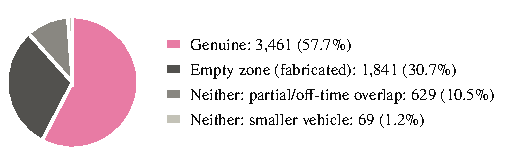
\includegraphics[width=\columnwidth]{fig_pie.pdf}
\caption{Composition of the main benchmark (6,000 scenes) by ground truth. Error rates are computed on genuine and empty-zone claims; the two ``neither'' groups are reported separately (Section~\ref{sec:graded}). Simulated data.}
\label{fig:pie}
\end{figure}


\subsection{Sanity Checks}
Before the benchmarks, on an earlier configuration of the formal tier, known-answer scenes were verified; an ideal-sensor run was compared with geometric visibility (no false refutation or support in 300 scenes; its 8 disagreements, all on curved roads, were abstentions explained in Section~\ref{sec:strata}); the road-frame geometry was checked by a round trip; the baselines were shown to be independent of the formal-tier settings; and the bound was calibrated against the ray-traced simulator (Section~\ref{sec:calib}).

\subsection{Benchmarks}
\begin{itemize}
\item \emph{Main:} 6,000 scenes, nominal parameters (seeds \mbox{$7{\times}10^6{+}i$}).
\item \emph{Degradation:} 13 conditions of 1,000 scenes with shared seeds \mbox{$8{\times}10^6{+}i$}: returns $-3$, $-6$ and $-9$~dB; persistent fade 6 and 8~dB; ghost rate 0.1 and 0.3; blockage (probability 0.3, flag recall 0.5); misalignment (probability 0.3, calibration noise $2^\circ$); clock $\sigma = 0.3$~s; pose noise 0.3~m and $1^\circ$; up to 12 vehicles; and a combined condition ($-6$~dB, fade 6~dB, blockage).
\item \emph{Selected stress sets:} returns $-9$~dB and the combined condition, 10,000 scenes each (seeds \mbox{$10{\times}10^6{+}i$}). They were chosen \emph{because} the persistence-only baseline had failed there, and the two rules of the rule tier were designed after these failures had been seen; the stress sets are therefore development data for the rule tier.
\item \emph{Pre-registered generalization test:} code and analysis frozen before running, with SHA-256 hashes of the simulator, method and runner code recorded; the analysis script implements the recorded H1 and H2 definitions. One design change was made before the freeze after inspecting the clock-error degradation condition (the window-end check was made tolerant of $\Delta_{\mathrm{clk}}$); one amendment after the freeze fixed a simulator crash at high speed before any affected result existed. Four conditions not used in any design decision---G1 returns $-12$~dB; G2 returns $-3$~dB with fade 8~dB (a new combination of two swept factors); G3 ego speed 100--130~km/h; G4 rain in every scene with up to 12 vehicles---with 10,000 scenes each (seeds \mbox{$11{\times}10^6{+}i$}, shared by the four conditions, so that G1 and G2 contain the same scenes). Primary endpoint H1 (a single test): wrong refutations, formal vs.\ rule tier, pooled, exact two-sided McNemar test, $\alpha = 0.05$; no power analysis was made, and because both tiers had made no error in the main benchmark, H1 was unlikely to be decidable; it was kept as registered. H2: Wilson 95\% upper limit of the standard level's wrong-refutation rate below 0.1\%. Secondary: error--coverage curves, a matched-coverage comparison and per-condition counts. The freeze (October 8, 2026) followed all exploratory runs; when the amendment was made, results of G1 and G2 had been written but not inspected.
\item \emph{Far-edge test:} 2,000 scenes with the genuine claimant within 1~m of $g_{\max}$ (seeds \mbox{$12{\times}10^6{+}i$}); the far-edge clause of (\ref{eq:6}) was added after this test, so it is development data.
\item \emph{Owner attacks:} 3,000 scenes per attack (seeds \mbox{$13{\times}10^6{+}i$}): rotation of a rear radar by $1.0^\circ$--$1.9^\circ$ (below the $2^\circ$ limit) in every scene; silent blockage of a rear radar (flag never set) on an empty road and in traffic.
\item \emph{Bound calibration:} 4,000 genuine claims per model condition, without traffic or faults, in rain (seeds \mbox{$14{\times}10^6{+}i$}).
\item \emph{Ledger test:} 60 main-benchmark scenes embedded in a realistic stream (50~s of driving before, the enriched event and 60~min to the anchor) and eight attacks.
\end{itemize}

\subsection{Methods Compared}
\begin{itemize}
\item The \emph{formal tier} and the \emph{rule tier} of Section~\ref{sec:problem}, and the \emph{graded verdict} that combines them.
\item A \emph{persistence-only baseline}: the rule tier without the any-detection and motorcycle rules, reading the same detection log and refuting when the zone is covered and no persistent detection lies in $Z^-$; it is the closest analog here of a live check that a reported object lies in observed free space~\cite{b24,b25}.
\item The \emph{rule tier without the motorcycle rule}.
\item An \emph{early prototype}: fixed ego-frame zone, a weather-based confidence instead of a bound, and no attestation, persistence or enrichment.
\item \emph{Ablations} of the formal tier: claim-derived zone (replaced by a fixed ego-frame box), attestation, liveness, bound, persistence and enrichment.
\end{itemize}
Event recorders and dashcams are not compared numerically: in a no-contact event they record nothing, or nothing that survives until the claim (Section~\ref{sec:related}).

\subsection{Statistics}
Two-sided Wilson 95\% intervals~\cite{b46} are used for rates near zero (their upper limit is a one-sided 97.5\% bound), percentile bootstrap intervals~\cite{b47} (2,000 resamples, seed 12345) for coverage, exact McNemar tests~\cite{b48} for paired comparisons; Newcombe's hybrid score interval~\cite{b61} for paired differences of rates, a scene-clustered bootstrap where conditions share scenes, and exact one-sided Poisson tests for observed against expected misses. Holm's method~\cite{b49} adjusts the 21 main-benchmark tests (six ablations and the prototype against the formal tier on three metrics). Results outside the pre-registered test are exploratory; pooled degradation counts are descriptive because the conditions share seeds.

\section{Results}\label{sec:results}

\subsection{Main Benchmark (RQ1)}
Table~\ref{tab:main} summarizes the nominal benchmark. Every method except the early prototype is error-free there; the methods differ in how often they refute. The rule tier refutes more fabricated claims than the formal tier (331 fabricated claims refuted only by the rule tier, 60 only by the formal tier; exact McNemar $p = 1.7 \times 10^{-46}$, unadjusted). The formal tier refutes 17.6\% of fabricated motorcycle claims, which the rule tier never refutes, and 61.1\% of car claims against the rule tier's 82.5\%. Genuine claims were SUPPORTED in 99.7\% (formal tier) and 99.9\% (rule tier) of cases and otherwise left INCONCLUSIVE. The prototype is unsafe in both directions (Holm-adjusted $p = 1.8 \times 10^{-12}$ and $2.2 \times 10^{-142}$ against the formal tier).

\begin{table*}[!t]
\centering
\footnotesize
\caption{Main Benchmark (Exploratory): Nominal Parameters, 6,000 Scenes (3,461 Genuine, 1,841 Empty, 698 Neither)}
\label{tab:main}
\renewcommand{\arraystretch}{1.15}
\begin{tabular}{>{\raggedright\arraybackslash}p{4.6cm}>{\raggedright\arraybackslash}p{3.4cm}>{\raggedright\arraybackslash}p{3.4cm}>{\raggedright\arraybackslash}p{3.6cm}}
\toprule
\textbf{Method} & \textbf{Wrong refutations$^{a}$ ($n = 3{,}461$)} & \textbf{Wrong supports$^{a}$ ($n = 1{,}841$)} & \textbf{Coverage [95\% CI]$^{b}$} \\
\midrule
Rule tier & 0 ($\le$ 0.11\%) & 0 ($\le$ 0.21\%) & 68.4\% [66.3, 70.6] \\
Formal tier & 0 ($\le$ 0.11\%) & 0 ($\le$ 0.21\%) & 53.7\% [51.4, 56.1] \\
Graded verdict, standard (both tiers refute) & 0 ($\le$ 0.11\%) & 0 ($\le$ 0.21\%) & 50.5\% [48.2, 52.8] \\
Rule tier without motorcycle rule & 0 ($\le$ 0.11\%) & 0 ($\le$ 0.21\%) & 82.4\% [80.6, 84.2] \\
Persistence-only baseline & 0 ($\le$ 0.11\%) & 0 ($\le$ 0.21\%) & 95.2\% [94.1, 96.1] \\
Early prototype & 44 (1.27\%) & 476 (25.9\%) & 48.7\% [46.3, 50.8] \\
\bottomrule
\multicolumn{4}{l}{\scriptsize $^{a}$Zero counts with Wilson 95\% upper limits; nonzero counts with point estimates. $^{b}$Percentile bootstrap.}
\end{tabular}
\end{table*}

\subsection{Ablations (RQ2)}\label{sec:ablation}
Table~\ref{tab:ablation} removes one component at a time from the formal tier. The claim-derived zone, persistence and attestation carry the safety at nominal conditions; liveness matters only under attack (Section~\ref{sec:attacks}) and the bound only under model mismatch (Section~\ref{sec:degr}). Enrichment raised formal-tier coverage from 49.4\% to 53.7\%, a net gain made of 191 fabricated claims refuted only with enrichment and 112 only without it, and raised the support of genuine claims from 96.2\% to 99.7\%; in the 188 genuine scenes in which the trigger was missed, the formal tier supported 97.3\% and the rule tier 100\%.

\begin{table*}[!t]
\centering
\footnotesize
\caption{Ablations (Exploratory): One Component Removed From the Formal Tier (Exact McNemar Against the Full Tier, Holm-Adjusted Over the 21-Test Family)}
\label{tab:ablation}
\renewcommand{\arraystretch}{1.15}
\begin{tabular}{>{\raggedright\arraybackslash}p{3.2cm}>{\raggedright\arraybackslash}p{2.4cm}>{\raggedright\arraybackslash}p{2.4cm}>{\raggedright\arraybackslash}p{1.6cm}>{\raggedright\arraybackslash}p{6.1cm}}
\toprule
\textbf{Removed component} & \textbf{Wrong refutations} & \textbf{Wrong supports} & \textbf{Coverage} & \textbf{Holm-adjusted $p$ (metric)} \\
\midrule
None & 0 & 0 & 53.7\% & --- \\
Claim-derived zone & 28 (0.81\%) & 472 (25.6\%) & 41.8\% & $1.1\times 10^{-7}$ (WR); $3.3\times 10^{-141}$ (WS); $1.4\times 10^{-40}$ (cov.) \\
Attestation & 0 & 18 (0.98\%) & 54.4\% & $9.9\times 10^{-5}$ (WS) \\
Liveness & 0 & 0 & 53.7\% & 1.0 (all metrics) \\
Miss bound & 0 & 0 & 62.6\% & $3.1\times 10^{-48}$ (cov.) \\
Persistence & 0 & 188 (10.2\%) & 53.7\% & $9.7\times 10^{-56}$ (WS) \\
Enrichment & 0 & 0 & 49.4\% & $9.3\times 10^{-5}$ (cov.) \\
\bottomrule
\multicolumn{5}{l}{\scriptsize WR: wrong refutations; WS: wrong supports; cov.: coverage. All metrics with adjusted $p < 0.05$ are listed.}
\end{tabular}
\end{table*}

\subsection{Pre-Registered Generalization Test (RQ3)}\label{sec:prereg}
The test comprised 40,000 new scenes under four unseen degradations (24,993 genuine and 10,551 empty claims).
\begin{itemize}
\item \textbf{H1 could not be decided.} The formal tier made 5 and the rule tier 6 wrong refutations; the tiers disagreed on a single genuine claim (wrong only for the rule tier), so the exact McNemar test ($p = 1.0$) had no power at these error rates. The paired difference in wrong-refutation rate was $-0.004$ percentage points (95\% CI $-0.024$ to $+0.014$): read post hoc, the test excludes differences larger than about 0.02 points but cannot show that either tier is safer. The six failed claims (five failed by both tiers, one by the rule tier only) come from four distinct scenes, all cars with weak returns: 2 in G1 ($-12$~dB), 3 in G2 ($-3$~dB, fade 8~dB), 1 in G3 (rule tier only) and none in G4; the two G1 failures recur in G2, which shares its scenes.
\item \textbf{H2 met as registered, but not in every condition.} Standard refutations were wrong for 5 of 24,993 genuine claims (0.020\%; Wilson 95\% upper limit 0.047\%). This pooled limit treats the scenes as independent although the conditions share seeds; per condition, the upper limits were 0.12\% (G1, 2 of 5,904), 0.15\% (G2, 3 of 5,904), 0.059\% (G3) and 0.058\% (G4), so the 0.1\% criterion is not met within G1 and G2. Weak-or-better refutations were wrong for 6 (0.024\%; upper limit 0.052\%). At this test's mix of genuine and empty claims (``neither'' claims excluded), 5 of 4,373 standard refutations (0.11\%) and 6 of 7,771 weak-or-better refutations (0.08\%) were wrong; this share depends on the base rate of fabricated claims.
\item \textbf{Coverage and support.} Neither tier made a wrong support. Coverage was 71.2\% for the rule tier, 43.8\% for the formal tier and 41.4\% at the standard level (scene-clustered 95\% CIs [69.7, 72.6], [42.5, 45.1] and [40.1, 42.7]). Of the 4,456 ``neither'' claims, the formal tier refuted 9 and the rule tier 25, 9 of them in G3. Genuine claims were SUPPORTED in 99.5\% (rule tier) and 99.2\% (formal tier) of cases. At high speed the claimed zone approaches the rear radars' 80~m range and formal-tier coverage falls to 6.9\% (rule tier 70.7\%).
\item \textbf{Error--coverage (Fig.~\ref{fig:errcov}).} At no $\varepsilon$ does the formal tier reach the rule tier's coverage with fewer errors; it reaches zero errors only at $\varepsilon = 10^{-6}$, with 25.0\% coverage. The rule tier is insensitive to the persistence count ($k_s = 2$--6 all give 6 errors at 71.2\%) because any in-zone detection already blocks refutation; without the motorcycle rule it makes 30 errors, and the persistence-only baseline 94.
\item \textbf{Matched coverage.} The pre-registered matched-coverage comparison could not be made as planned: the formal tier's coverage peaks at 57.7\% ($\varepsilon = 10^{-1}$, 28 errors), below the rule tier's 71.2\% (6 errors), and the rule tier cannot be tuned down because its coverage does not depend on $k_s$. At unequal coverage, the formal tier made fewer errors than the rule tier only at $\varepsilon \le 10^{-3}$ (5, 5, 5, 1 and 0 errors at 43.8\% down to 25.0\% coverage) and more at every larger $\varepsilon$.
\end{itemize}

\begin{figure}[!t]
\centering
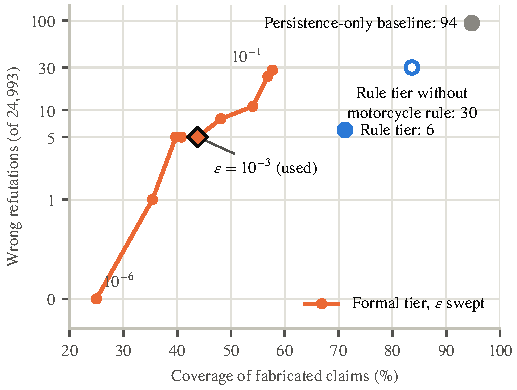
\includegraphics[width=\columnwidth]{fig_errcov.pdf}
\caption{Pre-registered generalization test (G1--G4 pooled; 24,993 genuine and 10,551 empty claims): wrong refutations (symmetric-log scale) against coverage of fabricated claims. The formal tier is swept over $\varepsilon \in \{10^{-1}, 3\cdot10^{-2}, 10^{-2}, 3\cdot10^{-3}, 10^{-3}, 3\cdot10^{-4}, 10^{-4}, 10^{-5}, 10^{-6}\}$; the diamond marks the operating point $\varepsilon = 10^{-3}$. The rule tier gives the same point for persistence counts $k_s = 2$--6. Simulated data.}
\label{fig:errcov}
\end{figure}


\subsection{Degradation, Stress Sets and the Zone Edge}\label{sec:degr}

\begin{figure}[!t]
\centering
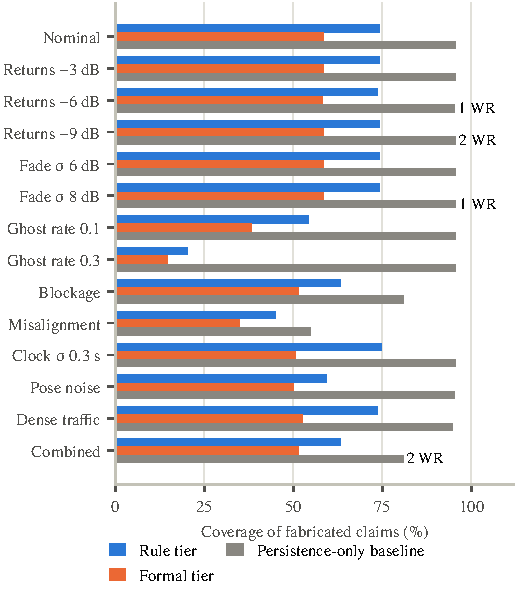
\includegraphics[width=\columnwidth]{fig_degr.pdf}
\caption{Coverage of fabricated claims in the 13 degradation conditions and a 1,000-scene nominal reference with the same seeds (its formal-tier coverage of 58.6\% differs from the 53.7\% of the 6,000-scene benchmark in Table~\ref{tab:main}). Labels mark wrong refutations (WR); the rule and formal tiers made none. Simulated data.}
\label{fig:degr}
\end{figure}


\textbf{Degradation conditions} (Fig.~\ref{fig:degr}; 1,000 scenes each, pooled 7,631 genuine and 3,796 empty claims). The formal tier made 0 wrong refutations and 0 wrong supports; the rule tier 0 and 2 (both under pose noise); the persistence-only baseline 6 and 2; the formal tier without the bound 2 and 0; and the prototype 156 and 928. Coverage falls most with ghosts (ghost rate 0.3: formal tier 14.8\%, rule tier 20.2\%) and misalignment (35.0\% and 45.1\%). Under weaker returns or heavier fading, coverage changes by at most 0.4 points for every method: an empty zone contains nothing whose detection depends on return strength, and the formal tier evaluates its bound under the nominal model in every condition. These conditions differ only in their wrong refutations.

\textbf{Stress sets} (Table~\ref{tab:stress}; exploratory). No method in the table made a wrong support; the early prototype, not shown, made 99 and 104 wrong refutations and 745 and 734 wrong supports. The persistence-only baseline's 49 failures were 41 motorcycles and 8 cars, and its deficit against the formal tier ($p = 6.0 \times 10^{-8}$ and $4.8 \times 10^{-7}$, unadjusted) is what the two rules of the rule tier were designed to remove; the rule tier's results here are therefore in-sample. Within the formal tier, the bound prevents 6 and 7 wrong refutations ($p = 0.031$ and $0.016$, unadjusted). Both tiers fail on the same two cars, at 35--39~m with a persistent fade near $-17$~dB. Genuine claims were SUPPORTED in 98.7\% (rule tier) and 98.4\% (formal tier) of cases in the combined condition.

\begin{table}[!t]
\centering
\footnotesize
\caption{Stress Sets (Exploratory; 5,910 Genuine and 2,926 Empty Claims Each): Wrong Refutations / Coverage}
\label{tab:stress}
\renewcommand{\arraystretch}{1.15}
\begin{tabular}{>{\raggedright\arraybackslash}p{3.4cm}>{\raggedright\arraybackslash}p{1.9cm}>{\raggedright\arraybackslash}p{1.9cm}}
\toprule
\textbf{Method} & \textbf{Returns $-9$~dB} & \textbf{Combined} \\
\midrule
Rule tier & 0 / 70.7\% & 2 / 61.6\% \\
Formal tier & 0 / 55.1\% & 2 / 48.1\% \\
Graded verdict, standard & 0 / 52.0\% & 2 / 45.6\% \\
Formal tier without bound & 6 / 62.7\% & 9 / 54.8\% \\
Rule tier without motorcycle rule & 6 / 82.9\% & 8 / 72.2\% \\
Persistence-only baseline & 25 / 94.4\% & 24 / 81.5\% \\
\bottomrule
\end{tabular}
\end{table}

\textbf{Far-edge test} (genuine claimant within 1~m of $g_{\max}$; 1,156 genuine and 599 empty claims). An earlier version of the free predicate (\ref{eq:6}), which accepted a return within $\delta$ of the far zone edge as free, made 4 wrong refutations; the formal tier with (\ref{eq:6}), whose far-edge clause was added in response, made 0 (coverage 56.1\%; in-sample), the rule tier 0 (70.6\%) and the persistence-only baseline 100, because its 0.5~m inset ignores returns at the edge.

\subsection{Calibration of the Miss Bound}\label{sec:calib}

\begin{figure*}[!t]
\centering
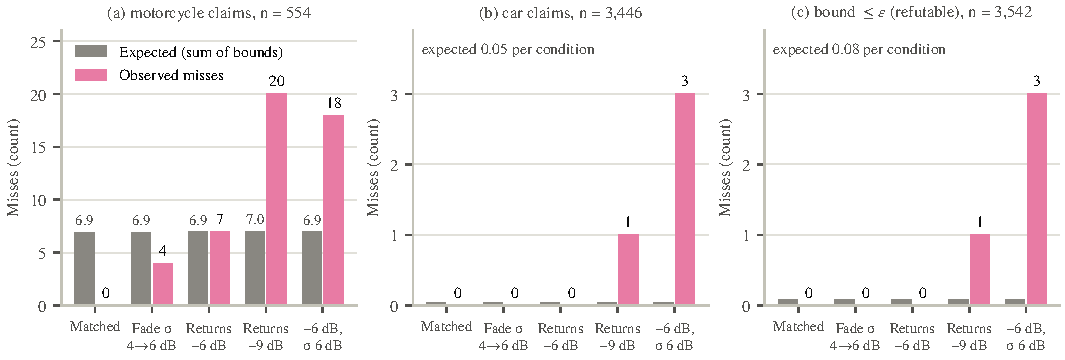
\includegraphics[width=\textwidth]{fig_calib.pdf}
\caption{Calibration of the miss bound against the ray-traced simulator (4,000 genuine claims per model condition; no traffic or faults; rain). Conditions: matched model; persistent-fade spread $\sigma_u$ raised from 4 to 6~dB; returns 6 or 9~dB weaker than modeled; returns 6~dB weaker with $\sigma_u = 6$~dB. Expected misses are the sum of the per-claim bounds, which the verifier computes under its nominal model in every condition; observed misses are claims for which every sample was free. (a) Motorcycle claims. (b) Car claims. (c) Claims whose bound is at most $\varepsilon$, i.e., the claims the formal tier would refute; all observed misses there were cars. Simulated data.}
\label{fig:calib}
\end{figure*}


Fig.~\ref{fig:calib} compares the bound with the misses observed in the simulator, by claimed class. The expected count is the sum of the per-claim bounds, which the verifier always computes under its nominal model; it therefore changes little between conditions (only through the sensor counts). Under the matched model no miss occurred in either class. \emph{Motorcycle claims} (Fig.~\ref{fig:calib}a) carry almost all of the expectation (6.9 of 7.0 per condition), and only 102 of the 554 have a bound $\le \varepsilon$. Observed misses were 4 with the persistent-fade spread raised from 4 to 6~dB, 7 with returns 6~dB weaker, and 20 and 18 with returns 9~dB weaker or 6~dB weaker with a 6~dB fade spread, 2.6--2.9 times the expectation ($p = 4 \times 10^{-5}$ and $3 \times 10^{-4}$, exact one-sided Poisson); none of these misses had a bound $\le \varepsilon$. \emph{Car claims} (Fig.~\ref{fig:calib}b) expect 0.05 misses per condition; 1 occurred at $-9$~dB and 3 in the combined condition, 22 and 65 times the expectation ($p = 0.045$ and $1.5 \times 10^{-5}$). Where the formal tier actually refutes, at bounds $\le \varepsilon$ (Fig.~\ref{fig:calib}c), the bound predicted 0.08 misses per condition, and the observed misses were exactly these four misses, from three distinct cars (bounds $4 \times 10^{-6}$, $8 \times 10^{-6}$ and, for the car missed in both conditions, $6.2 \times 10^{-4}$). The bound is therefore optimistic by more than an order of magnitude for weakly reflecting cars once the model is about 9~dB too optimistic. It was conservative for motorcycles under the matched model (0 misses against 6.9 expected); for cars, an expectation of 0.05 per condition is too small to show conservatism.

A sensitivity re-run with the no-return clause of (\ref{eq:6}) tightened to $d_i \ge r_i^{\max}$ (closer to A2) changed no formal-tier verdict in the 56,000 scenes of the main benchmark, the four pre-registered conditions and the combined stress set, including G3, where the zone approaches the range limit.

\subsection{Graded Verdict and Unclear Claims}\label{sec:graded}
The graded verdict keeps most of the rule tier's coverage while marking which refutations both tiers agree on: in the pre-registered test, 73.6\% of fabricated claims were refuted at least weakly and 41.4\% at the standard level. Requiring agreement added no safety over the formal tier alone in that test, because the formal tier's five wrong refutations were also made by the rule tier. Of the 698 ``neither'' claims, 69 have a smaller vehicle than claimed in the zone and 629 a partial or off-time overlap. The formal tier supported 689 and left 9 INCONCLUSIVE; the rule tier supported 689, left 7 INCONCLUSIVE and refuted 2, both car claims with a partial or off-time overlap, where a refutation of the claimed position at the claimed time is defensible but should be reported with care. A conservative-model tier (returns 6~dB weaker, fade 6~dB), defined after the stress sets had been run and identical to the combined stress condition, made no wrong refutation in any set where it was evaluated (it was excluded from the pre-registered test) but refuted only 0.3--4.7\% of fabricated claims (3.4\% at nominal parameters); it is not part of the proposed system.

\subsection{Owner Attacks, Integrity and Cost (RQ1, RQ4)}\label{sec:attacks}
Table~\ref{tab:attacks} lists the owner attacks. Liveness defeats a covered radar, also on an empty road, because the claimant is seen by the other rear radar: without liveness, the formal tier made 14--15 and the persistence-only baseline 15--18 wrong refutations, and with liveness both made none. The rule tier was evaluated only with liveness. A rotation below the calibration limit causes no wrong refutation but 4--6 wrong supports in every method, because the rotated radar places an adjacent-lane vehicle in the zone.

\begin{table*}[!t]
\centering
\footnotesize
\caption{Owner Attacks (3,000 Scenes Each): Wrong Refutations / Wrong Supports / Coverage}
\label{tab:attacks}
\renewcommand{\arraystretch}{1.15}
\begin{tabular}{>{\raggedright\arraybackslash}p{3.0cm}>{\raggedright\arraybackslash}p{2.2cm}>{\raggedright\arraybackslash}p{2.3cm}>{\raggedright\arraybackslash}p{2.2cm}>{\raggedright\arraybackslash}p{2.6cm}>{\raggedright\arraybackslash}p{2.6cm}}
\toprule
\textbf{Attack} & \textbf{Formal tier} & \textbf{Formal tier, no liveness} & \textbf{Rule tier} & \textbf{Persistence-only baseline, with liveness} & \textbf{Persistence-only baseline, no liveness} \\
\midrule
None & 0 / 0 / 56.8\% & 0 / 0 / 56.8\% & 0 / 0 / 72.8\% & 0 / 0 / 96.1\% & 0 / 0 / 96.1\% \\
Rotation $1.0^\circ$--$1.9^\circ$ & 0 / 4 / 45.7\% & 0 / 4 / 45.7\% & 0 / 6 / 59.4\% & 0 / 6 / 81.0\% & 0 / 6 / 81.0\% \\
Silent blockage, empty road & 0 / 0 / 32.5\% & 14 / 0 / 68.2\% & 0 / 0 / 38.5\% & 0 / 0 / 47.3\% & 15 / 0 / 97.7\% \\
Silent blockage, traffic & 0 / 0 / 31.1\% & 15 / 0 / 61.4\% & 0 / 0 / 40.1\% & 0 / 0 / 49.4\% & 18 / 0 / 97.6\% \\
\bottomrule
\multicolumn{6}{l}{\scriptsize Each attack: 1,714 genuine and 923 empty claims (empty road: 1,464 and 1,156).}
\end{tabular}
\end{table*}

\textbf{Integrity.} After disclosure and verification, the formal-tier verdict equaled the full-record verdict in 60 of 60 scenes. Eight attacks on the free-space record were all detected: editing a hit sector to free (Merkle root mismatch); editing, rebuilding and re-signing with another key (signature); re-signing the chain with the stolen key after the anchor (anchor mismatch); withholding a zone sector, a whole sample, the last block of the window, or its first block together with all earlier headers, while supplying valid proofs for the rest (completeness check); and replaying a disclosed block so that its samples would count twice in the bound (duplicate check). The duplicate check was added after an internal audit of the package found that a replayed block was accepted and lowered the bound. The detection log, and hence the rule tier, was not tested: an owner who deleted in-zone detections from it could turn a genuine claim into a weak refutation.

\textbf{Cost.} The free-space record costs 2.45~MB per hour at base resolution (headers, layouts and seeds included), for example 74~MB for 30 days with one hour of driving a day, and 152~kB of leaves per 20~s enriched event. A disclosure for an enriched claim cost a median of 48.6~kB (56 claims; 1,009 leaves, 352 proof hashes and 61 headers, with the anchor one hour after the claim) and 16.3~kB at base resolution (4 claims). The header chain grows by 184~bytes per minute of driving between the claim and the next anchor; hourly anchoring keeps it at about 11~kB, whereas daily anchoring would add up to 265~kB. The detection log was not sealed; its storage is estimated in Section~\ref{sec:discussion}.

\subsection{Strata and Strategic Claims}\label{sec:strata}
Neither tier made a wrong refutation in any traffic-density band (1--2, 3--4 and 5+ vehicles, counting claimant and occluding van; 779, 933 and 1,749 genuine claims). Formal-tier coverage falls with density (59.6\%, 57.3\%, 45.8\%), the rule tier's much less (69.1\%, 69.9\%, 66.8\%); the prototype made 17, 12 and 15 wrong refutations. On curved roads, all disagreements with geometric visibility in the ideal-sensor check were conservative: an adjacent-lane vehicle sharing a sector with the zone shortens that sector's stored range. Coverage also depends on what the claimant chooses to claim. A fabricated motorcycle claim is never refuted by the rule tier or at the standard level; formal-tier coverage falls from 66.8\% for short claimed gaps ($g_{\max} < 32$~m) to 47--50\% for longer ones, and collapses at high speed (Section~\ref{sec:prereg}). A strategic claimant can therefore choose claims that are hard to refute, although not claims that are wrongly supported.

\subsection{Stress Tests of the Assumptions (Exploratory)}\label{sec:stress}
Run after all other results, these tests use a copy of the simulator with four added options that are off by default; with them off it reproduced the main-benchmark verdicts exactly (100 scenes). Each set has 2,000 scenes (seeds \mbox{$15{\times}10^6{+}i$}); Table~\ref{tab:stressx} lists the results.
\begin{itemize}
\item \emph{Occlusion outside the zone.} Claims start at $g_{\min} = 12.5$~m, and a truck drives 0.6--1.4~m behind the ego vehicle in the claimed lane, outside the zone, where it can hide the claimant. The formal tier refuted none of the 845 fabricated claims, because the truck's returns shorten every zone sector; the rule tier refuted 85.6\% of them although it could at best partly observe the zone, and wrongly refuted one genuine claim; the persistence-only baseline wrongly refuted 33. This is the case that separates the tiers, and the main benchmark did not contain an occluder outside the zone.
\item \emph{Claimant leaves the zone (A6).} Every claimant brakes at 6~m/s$^2$ from the claimed time. With genuine claimants near $g_{\max}$, so that they leave the zone within $W$, neither tier made a wrong refutation, because returns from the samples in which the claimant was still in the zone blocked both; genuine-claim support fell to 93.0\% (formal tier) and 81.7\% (rule tier), and the persistence-only baseline made 204 wrong refutations.
\item \emph{Partial attenuation attack.} The rear radar on the lane-change side was attenuated by 10~dB without a blockage flag. It still reported strong targets and so passed liveness; neither tier made a wrong refutation.
\item \emph{Fades correlated over time.} In the calibration setting of Section~\ref{sec:calib} (4,000 genuine claims each), per-sample fades following an AR(1) process with correlation 0.5 or 0.9 between consecutive samples produced no miss, against 0.08 expected at bounds $\le \varepsilon$ and 6.9 for motorcycles. Because the matched model already produced no miss, this test has little power, and it correlates only the per-sample fade $v$.
\end{itemize}

\begin{table}[!t]
\centering
\footnotesize
\caption{Stress Tests (Exploratory; 2,000 Scenes Each): Wrong Refutations / Coverage}
\label{tab:stressx}
\renewcommand{\arraystretch}{1.15}
\begin{tabular}{>{\raggedright\arraybackslash}p{2.9cm}>{\raggedright\arraybackslash}p{1.3cm}>{\raggedright\arraybackslash}p{1.3cm}>{\raggedright\arraybackslash}p{1.6cm}}
\toprule
\textbf{Set (genuine / empty)} & \textbf{Formal tier} & \textbf{Rule tier} & \textbf{Persistence-only baseline} \\
\midrule
Occlusion (1,128 / 845) & 0 / 0.0\% & 1 / 85.6\% & 33 / 100\% \\
Braking (1,182 / 579) & 0 / 58.2\% & 0 / 73.9\% & 0 / 96.0\% \\
Braking, far edge (1,182 / 579) & 0 / 58.2\% & 0 / 73.9\% & 204 / 96.0\% \\
Attenuation 10~dB (1,181 / 580) & 0 / 57.6\% & 0 / 72.9\% & 1 / 94.8\% \\
\bottomrule
\multicolumn{4}{l}{\scriptsize No method made a wrong support in these sets.}
\end{tabular}
\end{table}

\section{Discussion}\label{sec:discussion}

\subsection{What Carries the Safety}
Apart from the early prototype, most wrong refutations in this study came from the persistence-only baseline, which read ``no persistent detection'' as ``no vehicle''; outside the occlusion test, the tiers' own errors were weakly reflecting cars missed throughout the window, which defeated both tiers at their operating points; in the pre-registered test they were avoided only at $\varepsilon = 10^{-6}$, with 25.0\% coverage. Two simple rules remove the first kind: let any detection inside the zone block refutation, and never refute a weak reflector. Under the degradations of the pre-registered test the formal tier reached comparable safety by a principled route---it abstains wherever a miss is plausible---but abstained far more often, and the test could not separate the tiers. The occlusion stress test shows where they differ: behind a truck outside the zone, the rule tier refuted 85.6\% of fabricated claims about zones it could at best partly observe, and one genuine claim, while the formal tier abstained on all of them. The rule tier's coverage advantage therefore includes refutations that are not evidence. The formal tier's value is \emph{auditability} and occlusion-awareness: a refutation comes with the assumptions under which it could be wrong (A1--A6) and a number that a court or insurer can weigh. A verifier that uses the rule tier should at least require that the zone be observed, as the formal tier's free-space test does.

\subsection{What a Verdict Means}\label{sec:verdict}
The system answers one question---was a vehicle in the claimed zone during the claimed window---and nothing about fault, speed or injury. SUPPORTED means that a vehicle was observed there, not necessarily of the claimed class. INCONCLUSIVE means only that the record cannot decide, and must never be presented as evidence against the driver. The formal tier's $\varepsilon$ holds in two senses that should not be confused: over the pre-registered test its wrong-refutation rate (0.020\%) stayed below $\varepsilon$, but per refuted claim the calibration of Section~\ref{sec:calib} showed misses well above the bound once the model was 9~dB too optimistic. How often a refutation is correct also depends on the share of fabricated claims, which is unknown. In the reported scams the claimant may genuinely have been behind the vehicle; the system then supports the position, and evidence about the claimed maneuver, such as the following vehicle's range rate, would be the more relevant output (future work). Driver-facing wording such as ``Your car observed this lane area as empty for the whole claimed period'' or ``Your car could not observe this area'' needs a user study.

\subsection{Deployment Considerations}
The logger needs, per radar and sample, an azimuth clearance (Section~\ref{sec:method}), which current interfaces do not always expose; the healthy-sensor count $n_i$ is stored in two bits, enough for the three radars covering the rear here but not for five-radar layouts. Logging costs $O(N_{\mathrm{sec}} + R)$ per sample and one SHA-256 per leaf, well within a zonal controller, but it was not measured on embedded hardware. Keys must be provisioned per vehicle with a public-key infrastructure that verifiers trust, and the logger must run under measured boot. The detection log at 10~Hz would add an estimated 1.5--19~MB per hour before sealing (one detection per object and sensor, or one per $0.5^\circ$ ray; 6~bytes each plus a 4-byte header per sensor and sample), up to eight times the free-space record.

\subsection{Safety and Security Standards}
The system does not act on the vehicle, so functional-safety requirements for control functions~\cite{b51} do not apply directly; the hazard is a wrong verdict. Following the safety of the intended functionality (SOTIF) approach~\cite{b50}, weak reflectors, heavy persistent fading, ghosts, occlusion and miscalibration are triggering conditions, and the bound is a residual-risk argument valid only within its model. Key management, attestation and anchoring fall under vehicle cybersecurity management~\cite{b52,b56}; changes to the rules, the model or $\varepsilon$ are software updates~\cite{b53}, and a verdict must name the version used.

\subsection{Operational Design Domain}
The results cover multi-lane roads, lane-change claims against a following vehicle, and two rear-corner radars with one front radar. They do not cover pedestrians, cyclists, stationary objects, parking, junctions, close-range claims in front of the vehicle and---for the formal tier---speeds at which the claimed gap approaches the rear radars' range. Liveness relies on the overlap of the two rear radars behind the vehicle, where every simulated zone lay; zones seen by one radar only were not tested. The claim tolerance $\tau = 1$~s was not varied; claims timed only to the nearest minute would need longer windows and lower coverage.

\subsection{Privacy and Regulation}\label{sec:privacy}
The record holds no images and no identities, and only the zone sectors of one claim are disclosed. A disclosure still reveals the ranges of any other road user sharing those sectors, the ego trajectory during the window and, through the header chain, when the vehicle was driving until the anchor. Because enrichment is triggered by the vehicle's own solid-line crossings, the block layouts also time-stamp the owner's own violations; a disclosure reveals this for the claimed window. The detection log is close to an object list; how much of it a claim would require to disclose, and what that reveals, is open. The record is linked to an identifiable vehicle and is likely personal data under the General Data Protection Regulation (GDPR)~\cite{b54}; retention, purpose limitation and owner control need legal review. The EU Data Act~\cite{b55} may support owner-initiated access to vehicle-generated data. These are research observations, not legal advice.

\subsection{Threats to Validity}
\begin{itemize}
\item \emph{Internal.} Simulator and methods were written by the same author, and the methods' detection model equals the simulator's at nominal parameters. Degradations, a pre-registered test on unseen conditions, stress tests of the assumptions and internal reviews, assisted by the same AI system that wrote the code, reduce but do not remove this risk. The pre-registration was recorded in a private workspace, not with an external registry.
\item \emph{Construct.} Ground truth is geometric and asymmetric (genuine at the event time, empty over the window); 698 of 6,000 scenes are in neither class and are reported separately. The distribution of fabricated claims is a modeling choice, and claimed gaps ended 24--48~m behind the vehicle; short claims were not simulated separately. Simulated claims always refer to the vehicle's own crossing.
\item \emph{External.} The simulation is 2-D and radar-only, with lidar-like rays every $0.5^\circ$ rather than radar beams and detection lists; radar cross-sections are assumed; detection follows the model family of A5 in every condition except the correlated-fade test; ghosts are uniform rather than caused by geometry; mounting offsets and static clutter are ignored; no baseline from the literature, such as an evidential occupancy grid, was implemented; no real data are used.
\item \emph{Conclusion.} Error counts of the two tiers are small (0--6), so intervals are wide and the primary test was underpowered; only the pre-registered test is confirmatory.
\end{itemize}

\subsection{Limitations}
(i) The ledger covers only the free-space record; the detection log needed by the rule tier is not yet integrity-protected, and its cost is only estimated, so RQ4 is answered for the formal tier only. (ii) Where refutations happen (bound $\le \varepsilon$), the bound was optimistic for cars once returns were about 9~dB weaker than modeled (3 misses observed against 0.08 expected in the combined condition). (iii) A radar rotated just below the $2^\circ$ calibration limit causes wrong supports in every method; the zone is not widened by the admissible bearing error (A3), and a tighter limit or a larger lateral margin is needed. (iv) Liveness uses the whole event window; a causal trailing window must be specified. (v) Sector-level storage lets adjacent-lane vehicles shorten zone sectors, costing coverage on curves. (vi) Assumptions A1--A4 and A6 are not fully enforced by the implementation; in particular, $n_i$ counts any sensor with a ray in the sector. (vii) The rule tier does not reason about occlusion and refuted unobserved zones in the occlusion stress test. (viii) The rule tier and the far-edge clause were designed on the stress sets and the far-edge test; only the pre-registered test is out-of-sample for both tiers. (ix) The zone ablation replaces the claim-derived zone by a fixed box that ignores the heading change during the lane change, which overstates the zone's value against a heading-compensated box.

\subsection{Path to Real-World Evidence}\label{sec:realworld}
The detection model and the rules must be fitted to real radar. Public datasets with radar and annotated objects~\cite{b57,b58} can estimate the detection probability against range and class, the spread of persistent fades and their correlation over time; they cannot show staged claims or owner manipulation. A proving-ground campaign with standardized soft vehicle targets~\cite{b59}, a motorcycle target, occluding vehicles, blocked, attenuated and rotated sensors and known positions would then measure wrong-refutation rates directly, followed by a new pre-registered test with an external time stamp.

\section{Conclusion}
Delayed, no-contact injury claims ask a driver to prove that a vehicle was not somewhere. This paper formulated that task as proof of absence and proposed an image-free evidence system: a zone and window derived from the claim, sensor attestation and liveness, a signed record disclosed only for the zone with a check that nothing was withheld, and a graded verdict from two refutation tiers. In simulation:
\begin{itemize}
\item \textbf{RQ1:} both tiers refuted a majority of fabricated claims (rule tier 68\%, formal tier 54\%) with no wrong verdict on 5,302 classifiable nominal claims, at the assumed mix of claimed classes (a claimant who always claims a motorcycle is refuted only by the formal tier, in 17.6\% of cases). Only the formal tier's evidence is sealed and measured: the free-space record costs 2.45~MB per driving hour and about 49~kB per disclosed enriched claim with hourly anchoring; the detection log would add an estimated 1.5--19~MB per hour.
\item \textbf{RQ2:} the claim-derived zone, persistence and sensor attestation are each necessary; removing one produced wrong refutations or wrong supports (Holm-adjusted $p \le 9.9 \times 10^{-5}$).
\item \textbf{RQ3:} in a pre-registered test on 40,000 claims (35,544 classifiable) under unseen degradations, the two tiers made a similar number of wrong refutations (rule tier 6, formal tier 5), and the test could not separate them; the formal tier refuted far fewer fabricated claims (44\% vs.\ 71\%), and refutations agreed by both tiers were wrong for 0.020\% of genuine claims (pooled upper limit 0.047\%; up to 0.15\% within single conditions). With an occluder outside the zone, only the formal tier abstained on zones it could not fully observe.
\item \textbf{RQ4:} liveness turned 14--18 wrong refutations from a silently covered radar into none, a 10~dB attenuation caused none, and the ledger detected all eight edit, withholding and replay attacks on the free-space record; the detection log is not yet protected, and a radar rotated just below the calibration limit still causes wrong supports.
\end{itemize}
In simulation, a vehicle could answer most fabricated position claims with radar data it already processes, provided that the verifier derives the zone from the claim, trusts only healthy sensors, abstains on weak reflectors and refutes only space it observed; an explicit miss bound adds an auditable statement of risk and the occlusion-awareness that detection rules lack. Whether this holds on real radar, against strategic claimants and with real occluders and fading, is the open question, and Section~\ref{sec:realworld} sets out how to answer it.

\section*{Data and Code Availability}
The simulator, methods, ledger, analysis scripts, result files and pre-registration record are held privately until a decision on patent filing and can be made available to reviewers in confidence; they will be released with the paper (code under the MIT license; data and figures under CC BY 4.0). Five scripts, listed in the package, regenerate the numbers in Sections~\ref{sec:setup}--\ref{sec:discussion} from the result files, and another draws the data figures; the pre-registration record holds the SHA-256 hashes of the frozen simulator, method and runner code. No human participants, personal data or images of identifiable people were used; the news cases cited are public reports.

\section*{Acknowledgment}
Literature and patent searching, simulation and ledger code, statistical analysis, internal reviews and drafting were assisted by an AI system (Claude, Anthropic). The author designed the study and takes full responsibility for the content.
